% Chapter 4 (Results), restructured. Scope follows chapter3_final.tex.
% Tables between "% BEGIN AUTO" / "% END AUTO" are generated by build_chapter4_final.py;
% narrative figures were checked against chapter4_final_facts.json.
\documentclass[12pt,a4paper]{report}
\usepackage[T1]{fontenc}
\usepackage[utf8]{inputenc}
\usepackage[margin=25mm]{geometry}
\usepackage{amsmath,amssymb,booktabs,array,graphicx,tabularx}
\graphicspath{{figures/}{documents/thesis/figures/}}
\usepackage[round,authoryear]{natbib}
\usepackage[hidelinks]{hyperref}
\setlength{\emergencystretch}{3em}
\begin{document}
\setcounter{chapter}{3}
\chapter{Results}
\label{chap:results}

\section{Introduction}

This chapter reports the outcomes of the controlled experiments described in
Chapter~3 and uses them to answer the two research questions:
\begin{enumerate}
\item[\textbf{RQ1}] What are the effects of acoustic data-level curriculum
learning on the fine-tuning of ASR foundation models on limited Shona data?
\item[\textbf{RQ2}] How does combining curriculum schedulers with synthetic data
augmentation affect the out-of-domain generalisation of Shona ASR models?
\end{enumerate}

Section~\ref{sec:reading} sets out how the results should be read.
Section~\ref{sec:zero} establishes what fine-tuning itself achieves, and
Section~\ref{sec:overview} summarises all fine-tuned conditions.
Sections~\ref{sec:rq1} and~\ref{sec:rq2} answer RQ1 and RQ2 in turn.
Section~\ref{sec:cost} reports computational cost, and
Section~\ref{sec:summary} draws the findings together.

The principal findings are:
\begin{itemize}
\item Fine-tuning on roughly 80 hours of WAXAL speech transforms both models from
unusable zero-shot output (119--155\% WER) to 24--31\% WER on unseen WAXAL
speakers. This change is two orders of magnitude larger than any difference
between training strategies.
\item No curriculum reliably lowered final word error rate. Duration-sorted
SortaGrad caused a large temporary loss of accuracy after its first epoch, from
which every run recovered.
\item Light SpecAugment masking was the only intervention that improved Whisper
Medium on both the in-domain and the external test set. Combining it with a
curriculum did not add a measurable benefit.
\end{itemize}

\section{Reading the results}
\label{sec:reading}

Table~\ref{tab:conditions} lists the conditions reported in this chapter. Both
Whisper Base and Whisper Medium were trained under the shared conditions. The
dynamic curricula and the strict SNR ordering were screened with Whisper Base
only. Unless stated otherwise, each value is the mean over the three training
seeds (42, 43 and 44), with the sample standard deviation (SD) after $\pm$.

\begin{table}[htbp]\centering\small
\caption{Conditions reported in this chapter. All conditions use the
speaker-disjoint WAXAL protocol, three epochs and the fixed training and
decoding configuration of Chapter~3.}
\label{tab:conditions}
\begin{tabular}{llcc}\toprule
Code & Training condition & Base & Medium\\\midrule
% BEGIN AUTO conditions
C0 & Random order & \checkmark & \checkmark \\
C1 & SortaGrad & \checkmark & \checkmark \\
C2 & SNR order & \checkmark & -- \\
C3 & SNR+duration order & \checkmark & \checkmark \\
C5 & Loss-based (dynamic) & \checkmark & -- \\
C6 & WER-based (dynamic) & \checkmark & -- \\
A2 & Waveform + random & \checkmark & \checkmark \\
A3 & Waveform + SNR+duration & \checkmark & \checkmark \\
S2 & Light masks + random & \checkmark & \checkmark \\
S3 & Light masks + SortaGrad & \checkmark & \checkmark \\
S4 & Strong masks + random & \checkmark & \checkmark \\
S5 & Strong masks + SortaGrad & \checkmark & \checkmark \\
% END AUTO conditions
\bottomrule\end{tabular}
\end{table}

Four conventions apply throughout.
\begin{enumerate}
\item \textbf{Differences} are reported in percentage points (pp) as control WER
minus treatment WER, so positive values favour the treatment. They are computed
before rounding.
\item \textbf{Deterministic conditions.} Static orderings applied in every epoch
(C2 and C3) remove the only source of run-to-run randomness, which is the data
order. Their three seeds therefore produced identical predictions and constitute
one trained model, marked $\dagger$. By the same reasoning, the SD of the
random-order control C0 measures the effect of data order alone.
\item \textbf{Uncertainty.} For Whisper Medium, 95\% intervals come from a paired
cluster bootstrap with 100{,}000 resamples. It resamples the 24 WAXAL test
speakers, or the 348 FLEURS sentence prompts, keeping all recordings of a
resampled cluster together and applying the same resample to the control and the
treatment. These intervals describe uncertainty about the evaluation sample for
the trained models, not about new training runs. Most per-utterance Base
predictions were not retained, so Base differences are reported without
intervals.
\item \textbf{Model comparison.} Base was trained on an RTX~4090 and Medium on an
A100 (Chapter~3). Base--Medium differences therefore describe the two trained
systems, not the effect of model size alone. Every comparison \emph{within} a
model uses one GPU type; the original RTX~4090 Medium runs are compared with
their A100 repetitions in Appendix Table~\ref{tab:migration}.
\end{enumerate}

\section{Zero-shot performance and the effect of fine-tuning}
\label{sec:zero}

Table~\ref{tab:zero} compares each pretrained model, decoded with the Shona
language token and greedy decoding, against its fine-tuned random-order
control (C0).

\begin{table}[htbp]\centering\small
\caption{Test-set error rates (\%) before and after fine-tuning. Fine-tuned
values are C0 means over three seeds. The gain is zero-shot minus fine-tuned
WER in pp.}
\label{tab:zero}
\begin{tabular}{llrrrrr}\toprule
 & & \multicolumn{2}{c}{Zero-shot} & \multicolumn{2}{c}{Fine-tuned (C0)} & \\
\cmidrule(lr){3-4}\cmidrule(lr){5-6}
Corpus & Model & WER & CER & WER & CER & Gain\\\midrule
% BEGIN AUTO zero
WAXAL & Base & 132.2 & 57.2 & 31.0 & 6.8 & 101.1 \\
WAXAL & Medium & 119.1 & 95.7 & 23.8 & 4.5 & 95.3 \\
FLEURS & Base & 155.4 & 71.8 & 58.3 & 18.9 & 97.1 \\
FLEURS & Medium & 130.9 & 100.5 & 38.4 & 10.0 & 92.5 \\
% END AUTO zero
\bottomrule\end{tabular}
\end{table}

Fine-tuning reduced WAXAL test WER by 101.1~pp for Base and 95.3~pp for Medium,
relative reductions of 76.5\% and 80.0\%. On FLEURS, which played no part in
training or model selection, WER fell by 97.1~pp and 92.5~pp. Fine-tuning on
WAXAL therefore transferred to a corpus with different speakers, recording
conditions and text domain.

Figure~\ref{fig:zero-errors} shows that the two pretrained models fail in
different ways.
\begin{itemize}
\item \textbf{Base zero-shot} errors are mostly substitutions (88.7 per 100
reference words on WAXAL) plus many insertions. Base produces text of roughly
the right length, but almost every word is wrong.
\item \textbf{Medium zero-shot} errors are dominated by deletions (80.1 per 100
words on WAXAL and 84.2 on FLEURS). Inspection shows that its typical output is
a single repeated non-Latin character that runs until the length limit; the
median hypothesis contains one ``word''. Medium's lower zero-shot WER therefore
does not indicate better zero-shot recognition. Its CER (95.7\% on WAXAL) is
worse than Base's (57.2\%).
\end{itemize}
After fine-tuning, both models make mainly substitution errors, with few
deletions or insertions. The remaining errors are word-level misrecognitions,
not failures to produce Shona.

\begin{figure}[htbp]\centering
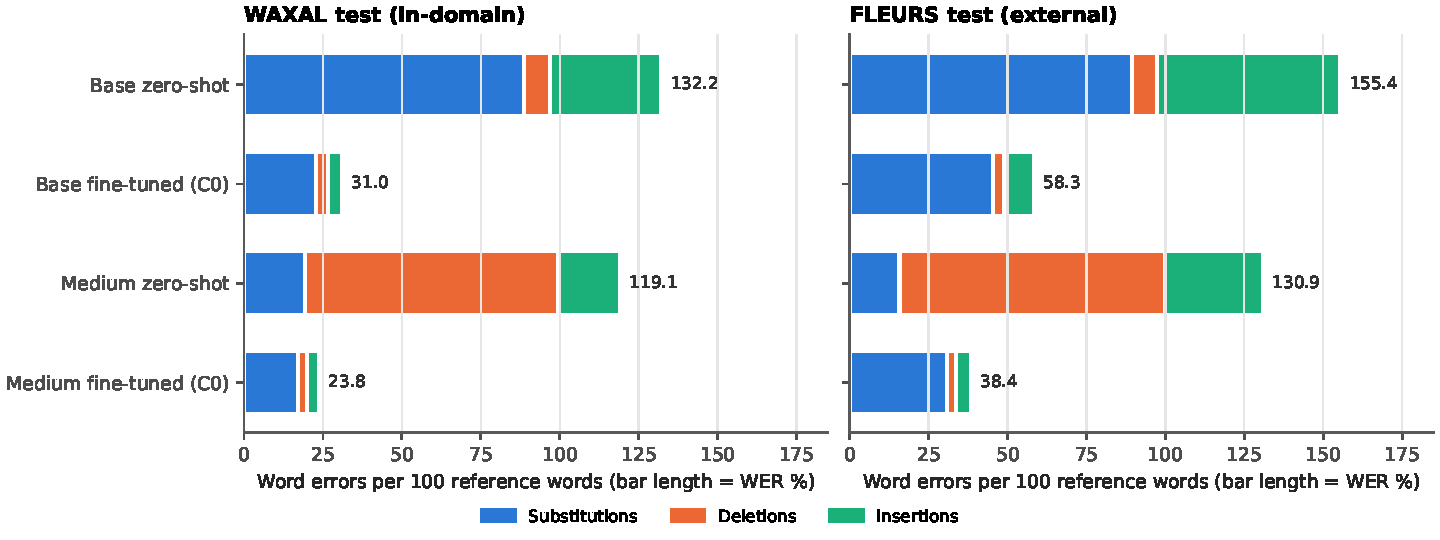
\includegraphics[width=\linewidth]{ch4_zero_shot_errors.pdf}
\caption{Composition of word errors before and after fine-tuning. Each bar
divides WER into substitutions, deletions and insertions per 100 reference
words. Fine-tuned bars are C0 means over three seeds.}
\label{fig:zero-errors}
\end{figure}

\section{Overview of the fine-tuned conditions}
\label{sec:overview}

Figure~\ref{fig:overview} shows test WER for every condition shared by the two
models; Table~\ref{tab:waxal} gives the WAXAL values. Two features dominate.
\begin{itemize}
\item The Medium system is better than the Base system in every condition. For
C0 the difference is 7.27~pp on WAXAL (31.04\% versus 23.78\%) and 19.95~pp on
FLEURS (58.31\% versus 38.36\%).
\item Within each model, the conditions span only 1.2--1.4~pp on WAXAL
(Base 30.20--31.37\%, Medium 22.42--23.82\%). Differences between
training strategies are small compared with the effect of model size or of
fine-tuning itself.
\end{itemize}
Medium's external error is still 14.6~pp higher than its in-domain error,
compared with 27.3~pp for Base. Domain shift remains substantial for both models.

\begin{figure}[htbp]\centering
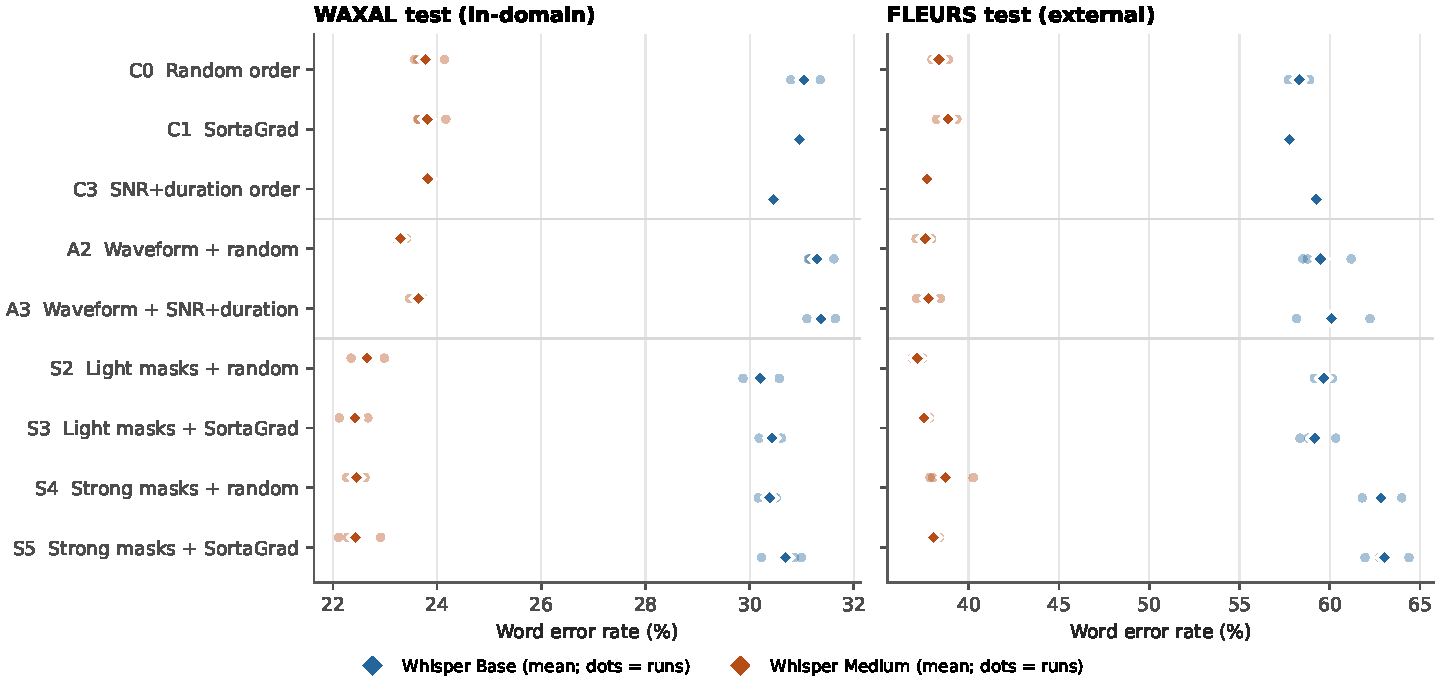
\includegraphics[width=\linewidth]{ch4_overview.pdf}
\caption{Test WER for the conditions shared by Whisper Base and Medium. Diamonds
are means; faint dots are individual training runs. C3 shows a single model
because its runs were identical. The horizontal axes differ between panels.}
\label{fig:overview}
\end{figure}

\begin{table}[htbp]\centering\scriptsize
\caption{WAXAL results (\%), mean $\pm$ SD over three seeds. $\dagger$:~identical
predictions across seeds (a single model). Validation WER was used to select the
checkpoint; test WER and CER are held-out results.}
\label{tab:waxal}
\setlength{\tabcolsep}{3pt}
\begin{tabular}{lrrrrrr}\toprule
 & \multicolumn{3}{c}{Whisper Base} & \multicolumn{3}{c}{Whisper Medium}\\
\cmidrule(lr){2-4}\cmidrule(lr){5-7}
Code & Val.\ WER & Test WER & Test CER & Val.\ WER & Test WER & Test CER\\\midrule
% BEGIN AUTO waxal
C0 & $32.91 \pm 0.48$ & $31.04 \pm 0.29$ & $6.82 \pm 0.17$ & $25.56 \pm 0.25$ & $23.78 \pm 0.32$ & $4.51 \pm 0.17$ \\
C1 & $32.60 \pm 0.11$ & $30.96 \pm 0.06$ & $6.89 \pm 0.12$ & $25.80 \pm 0.32$ & $23.81 \pm 0.31$ & $4.54 \pm 0.25$ \\
C3 & $32.84^{\dagger}$ & $30.46^{\dagger}$ & $6.47^{\dagger}$ & $25.77^{\dagger}$ & $23.82^{\dagger}$ & $4.36^{\dagger}$ \\
A2 & $33.06 \pm 0.24$ & $31.30 \pm 0.28$ & $7.12 \pm 0.22$ & $25.03 \pm 0.09$ & $23.30 \pm 0.10$ & $4.40 \pm 0.03$ \\
A3 & $33.04 \pm 0.34$ & $31.37 \pm 0.27$ & $7.10 \pm 0.15$ & $25.02 \pm 0.07$ & $23.64 \pm 0.14$ & $4.40 \pm 0.07$ \\
S2 & $31.76 \pm 0.16$ & $30.20 \pm 0.35$ & $6.71 \pm 0.45$ & $24.54 \pm 0.14$ & $22.65 \pm 0.32$ & $4.25 \pm 0.06$ \\
S3 & $32.20 \pm 0.26$ & $30.43 \pm 0.22$ & $6.89 \pm 0.26$ & $24.47 \pm 0.26$ & $22.42 \pm 0.28$ & $4.07 \pm 0.06$ \\
S4 & $32.46 \pm 0.28$ & $30.38 \pm 0.19$ & $6.93 \pm 0.28$ & $24.06 \pm 0.13$ & $22.45 \pm 0.18$ & $4.35 \pm 0.02$ \\
S5 & $32.41 \pm 0.08$ & $30.69 \pm 0.41$ & $7.09 \pm 0.30$ & $24.05 \pm 0.15$ & $22.44 \pm 0.43$ & $4.24 \pm 0.37$ \\
% END AUTO waxal
\bottomrule\end{tabular}
\end{table}

\section{RQ1: Curriculum learning}
\label{sec:rq1}

\subsection{Effect on final accuracy}

Figure~\ref{fig:base-curricula} compares the five curricula screened with
Whisper Base against the random-order control.

\begin{figure}[htbp]\centering
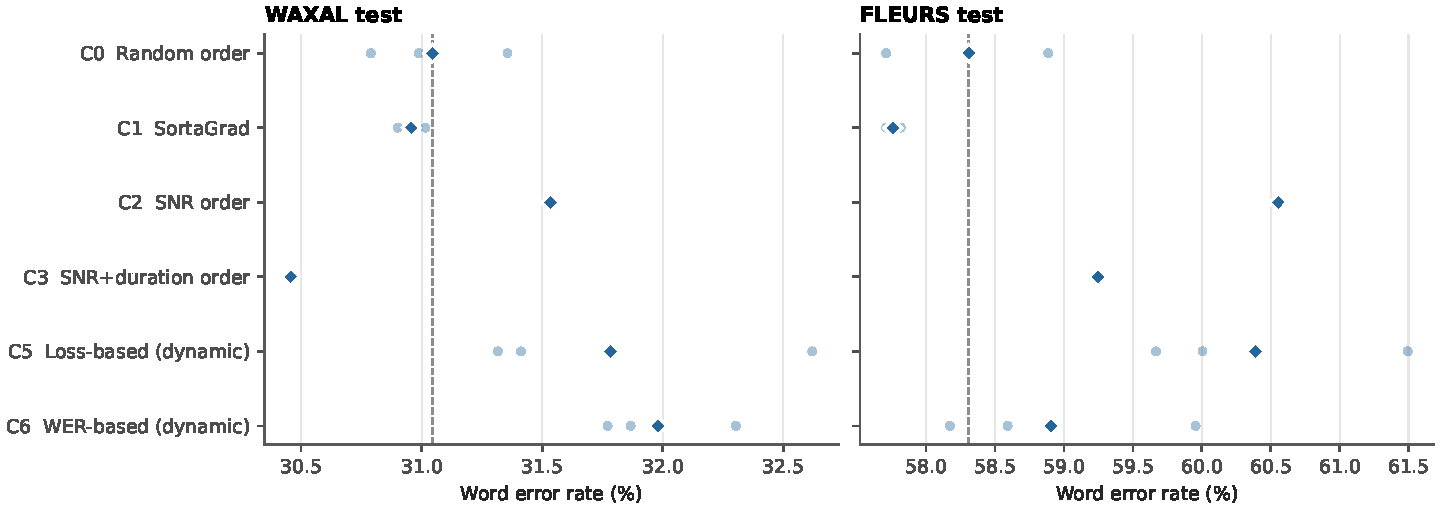
\includegraphics[width=\linewidth]{ch4_base_curricula.pdf}
\caption{Whisper Base test WER for the curriculum conditions. Diamonds are
means; faint dots are individual runs; the dashed line marks the C0 mean.
C2 and C3 each represent a single model. Values are given in Appendix
Table~\ref{tab:base-curricula}.}
\label{fig:base-curricula}
\end{figure}

\paragraph{Static curricula.} SortaGrad (C1) changed Base test WER by only
0.09~pp on WAXAL and 0.55~pp on FLEURS. The combined SNR and duration ordering
(C3) gave the lowest Base WAXAL test WER among the curricula (30.46\%, 0.59~pp
better than C0). The same model was 0.94~pp \emph{worse} than C0 on FLEURS, and
its validation WER barely differed from C0 (0.07~pp). Ordering by SNR alone
(C2) was worse than C0 on both corpora.

With Whisper Medium, neither static curriculum changed WAXAL test WER: C1 and C3
were each 0.04~pp worse than C0, with 95\% intervals of $[-0.36, 0.38]$ and
$[-0.40, 0.41]$~pp (Figure~\ref{fig:forest}). On FLEURS, C1 was 0.49~pp worse
and C3 0.68~pp better, again with intervals spanning zero. These effects are
an order of magnitude smaller than the order-only variation within C0
(SD 0.32~pp on WAXAL).

\paragraph{Dynamic curricula.} The loss-based (C5) and WER-based (C6) curricula,
which re-rank utterances by the model's own difficulty at each epoch, were worse
than C0 on WAXAL test WER by 0.73 and 0.94~pp. Neither improved FLEURS WER.
Both selected their epoch-2 checkpoint in every run. Their validation WER rose
during the third epoch (C6: 33.93\% to 34.98\%), while it continued to fall for
C0. When the hardest utterances are presented together at the end of training,
in-domain recognition got worse.

\subsection{Learning dynamics}

Final-checkpoint results hide how the curricula changed training.
Figure~\ref{fig:curves} shows validation WER at the end of each epoch.

\begin{figure}[htbp]\centering
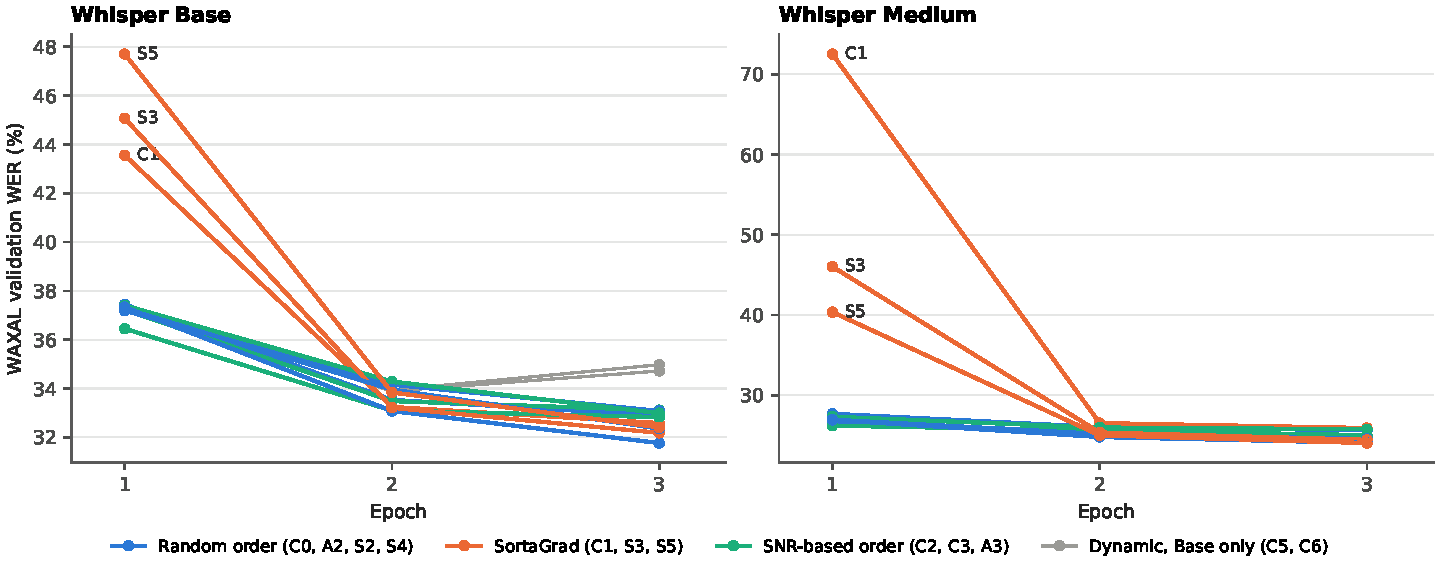
\includegraphics[width=\linewidth]{ch4_learning_curves.pdf}
\caption{WAXAL validation WER at the end of each epoch, averaged over seeds and
coloured by ordering family. The vertical scales differ between panels.}
\label{fig:curves}
\end{figure}

Three observations follow.
\begin{enumerate}
\item \textbf{SortaGrad degrades the model sharply after its first epoch.}
After an epoch of shortest-first training, Medium validation WER was 72.5\%,
compared with 27.7\% for random order; Base reached 43.6\% versus 37.4\%. The
model had learned from short utterances only and generalised poorly to the full
duration range. Validation decoding at this point took 93~minutes instead of
53, which is consistent with long, repetitive hypotheses. Once shuffled training
resumed, every SortaGrad run recovered within one epoch to the level of the
control.
\item \textbf{The SNR and duration ordering gives an early advantage that does
not persist.} C3 had the lowest epoch-1 validation WER for both models (Base
36.5\% versus 37.4\%; Medium 27.3\% versus 27.7\%), but the advantage had
disappeared by epoch 3. This is the faster early convergence that motivates
curriculum learning \citep{Bengio2009}, without a better end point.
\item \textbf{Most models were still improving at the final epoch.} Of the 62
runs with a recorded selection, 54 selected the final checkpoint. All comparisons
are therefore made at a fixed three-epoch budget, which limits both the early
effect of curricula and the late effect of regularisation.
\end{enumerate}

These dynamics explain the small final effects. SortaGrad was introduced to
stabilise the early optimisation of a network trained from random initialisation
\citep{Amodei2015}. When a pretrained recogniser is fine-tuned, the early
instability it addresses is largely absent. The cost of a length-biased first
epoch is then visible, but its benefit is not.

\subsection{Effect on difficult utterances}

The acoustic curricula define difficulty by duration and estimated SNR. They
could therefore help on difficult utterances even with little change in the
corpus mean. Figure~\ref{fig:bins} divides the Medium WAXAL test set into
thirds by each property and shows each condition's change relative to C0.

\begin{figure}[htbp]\centering
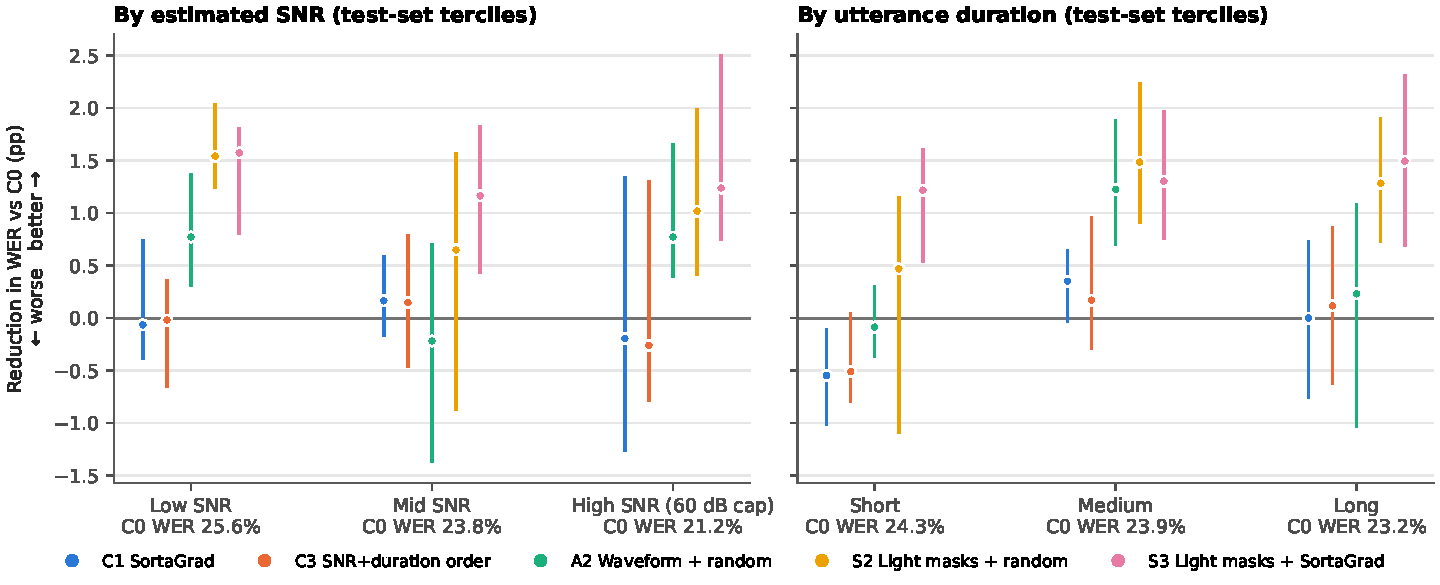
\includegraphics[width=\linewidth]{ch4_difficulty_bins.pdf}
\caption{Whisper Medium WAXAL test WER reduction relative to C0 within thirds of
the test set by estimated SNR (left) and duration (right). Points are means over
three seeds; bars are 95\% speaker-cluster bootstrap intervals. The highest SNR
third consists of recordings at the 60~dB cap. These 30 comparisons are
descriptive and are not adjusted for multiplicity.}
\label{fig:bins}
\end{figure}

Neither curriculum helped on the utterances it treats as hardest: on the
lowest-SNR third and the longest third, C1 and C3 were within 0.12~pp of C0.
Both were instead slightly worse on the shortest third, by about 0.5~pp, even
though SortaGrad presents short utterances first. In contrast, light masking
(S2, S3) had positive point estimates in every third, including about 1.5~pp on the noisiest
recordings. The absence of a curriculum benefit is therefore not concealed by
averaging over the test set.

\subsection{Answer to RQ1}

Under a fixed three-epoch fine-tuning budget, acoustic curricula did not
reliably change the final recognition accuracy of either Whisper model on
unseen Shona speakers or on external speech. Where a curriculum improved one
test set, it worsened the other (Base and Medium C3). Model-based dynamic
curricula were less accurate than random order and cost considerably more
(Section~\ref{sec:cost}). The curricula did change the course of training:
SortaGrad caused a temporary but severe loss of accuracy, and the SNR and
duration ordering gave a short-lived early advantage.

\section{RQ2: Augmentation and its combination with curricula}
\label{sec:rq2}

Figure~\ref{fig:forest} summarises every matched comparison on both test sets.
The rows separate the effect of augmentation alone (A2 and S2 against C0, and
S3 against C1) from the effect of adding a curriculum to augmented training
(A3 versus A2, S3 versus S2) and the effect of stronger masking (S4 versus S2,
S5 versus S3). The numerical values
are given in Appendix Table~\ref{tab:effects}.

\begin{figure}[htbp]\centering
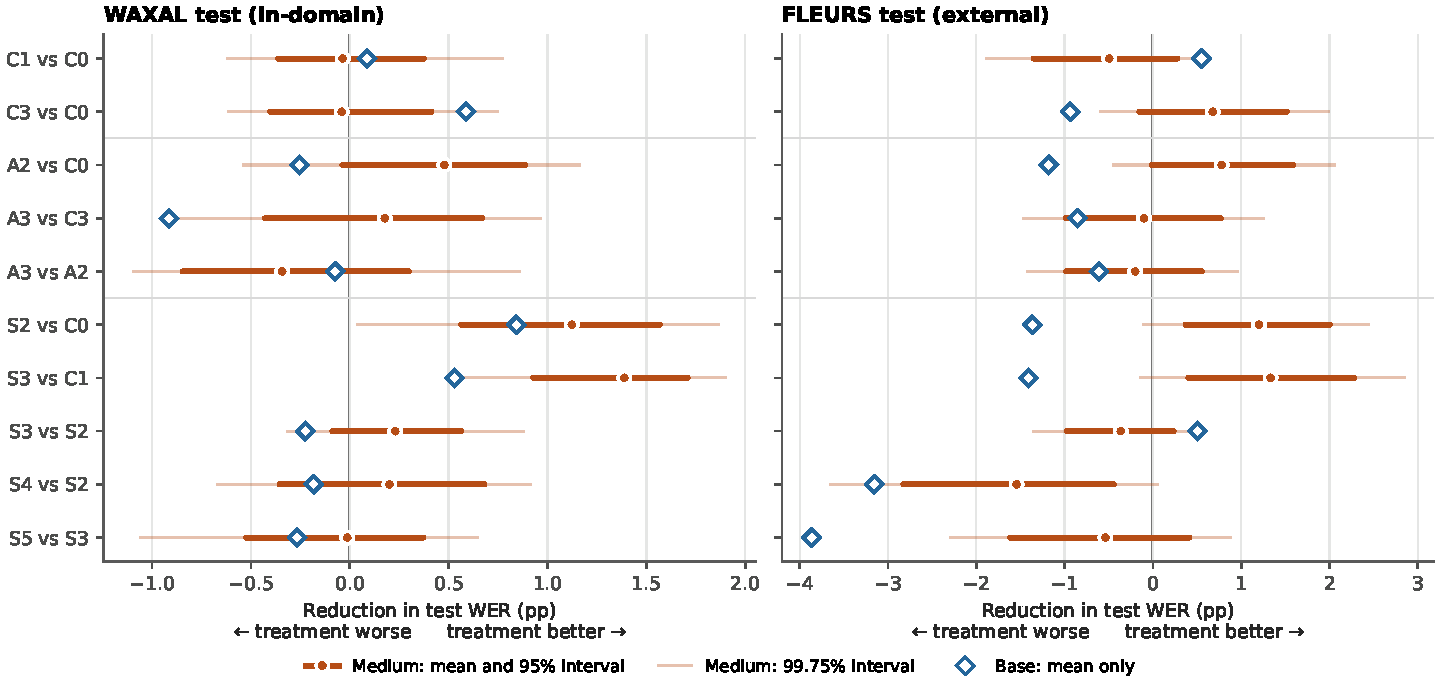
\includegraphics[width=\linewidth]{ch4_effects_forest.pdf}
\caption{Matched test-WER differences (control minus treatment, pp); positive
values favour the treatment. For Whisper Medium, thick bars are 95\% paired
cluster-bootstrap intervals and thin bars are 99.75\% intervals, which
correspond to a Bonferroni adjustment for the 20 comparisons shown. Base values
are means without intervals.}
\label{fig:forest}
\end{figure}

\subsection{Augmentation without a curriculum}

\paragraph{Waveform augmentation.} Additive noise, simulated reverberation and
tempo perturbation (A2) affected the two models in opposite directions. It made
Base worse on both test sets, by 0.25~pp on WAXAL and 1.18~pp on FLEURS. For
Medium it improved WAXAL WER by 0.48~pp $[-0.04, 0.89]$ and FLEURS WER by
0.78~pp $[-0.01, 1.59]$, with improvements for all three seeds on both sets. The
Medium intervals only just include zero, so the benefit is probable but not
established.

\paragraph{Spectrogram masking.} Light masking (S2) gave the clearest benefit of
any intervention. For Medium it reduced WAXAL WER by 1.12~pp $[0.56, 1.57]$, a
4.7\% relative reduction, and FLEURS WER by 1.20~pp $[0.37, 2.00]$, a 3.1\%
relative reduction. Every seed improved on both sets. The in-domain gain remains
positive under the 20-comparison adjustment $[0.04, 1.86]$; the external
interval then just includes zero $[-0.10, 2.44]$. For Base, S2 also gave the
lowest WAXAL test WER (30.20\%, 0.84~pp better than C0), but it was 1.36~pp worse
on FLEURS.

Stronger masking (S4: two time and two frequency masks) did not improve on light
masking in-domain for either model. It made external performance worse:
Medium FLEURS WER was 1.54~pp higher than S2 $[0.44, 2.83]$, and Base FLEURS WER
3.15~pp higher. \citet{Park2019} favoured the stronger LD policy for
large-scale English training. With 80~hours of Shona and a pretrained model,
the milder policy generalised better.

\subsection{Adding a curriculum to augmented training}

Adding a curriculum did not improve augmented training in any comparison whose
interval excludes zero.
\begin{itemize}
\item \textbf{Waveform augmentation with C3 ordering (A3).} Medium WAXAL WER was
0.34~pp worse than A2 $[-0.84, 0.30]$, with all three seeds worse, and FLEURS
WER was 0.20~pp worse. Base was also worse on both sets.
\item \textbf{Light masking with SortaGrad (S3).} S3 gave Medium's lowest mean
WAXAL WER (22.42\%), 0.23~pp better than S2 $[-0.09, 0.56]$, but one of the three
seeds was worse. On FLEURS it was 0.36~pp worse than S2 $[-0.98, 0.24]$. With
Base it was worse than S2 in-domain and better externally.
\end{itemize}

The interaction asks whether the curriculum's effect changes when augmentation
is present: (A2$-$A3)$-$(C0$-$C3) for waveform augmentation and
(S2$-$S3)$-$(C0$-$C1) for masking. For Medium on WAXAL these were $-0.30$~pp
$[-0.88, 0.21]$ and $+0.27$~pp $[-0.22, 0.68]$. On FLEURS they were $-0.88$~pp
$[-1.98, 0.19]$ and $+0.13$~pp $[-0.78, 1.08]$. No interaction is
distinguishable from zero, and none is consistently positive across the two
test sets.

The learning curves do show one interaction. Masking softened SortaGrad's
first-epoch degradation in Medium, where epoch-1 validation WER was 46.0\% for
S3 and 40.4\% for S5 against 72.5\% for C1. It did not do so in Base. Masking
appears to reduce the model's over-specialisation to short utterances. This
does not, however, lead to a better final model.

\subsection{Out-of-domain generalisation}

Table~\ref{tab:fleurs} and Figure~\ref{fig:domain} relate in-domain and
external performance. Every Base condition that improved WAXAL WER worsened
FLEURS WER, except SortaGrad, which lay only marginally below the control on
both axes. For Medium, every augmented
condition except S4 improved on C0 on both test sets, with S2 best externally
and S3 best in-domain. An in-domain ranking is therefore not a reliable guide
to the external ranking, particularly for the smaller model.

\begin{figure}[htbp]\centering
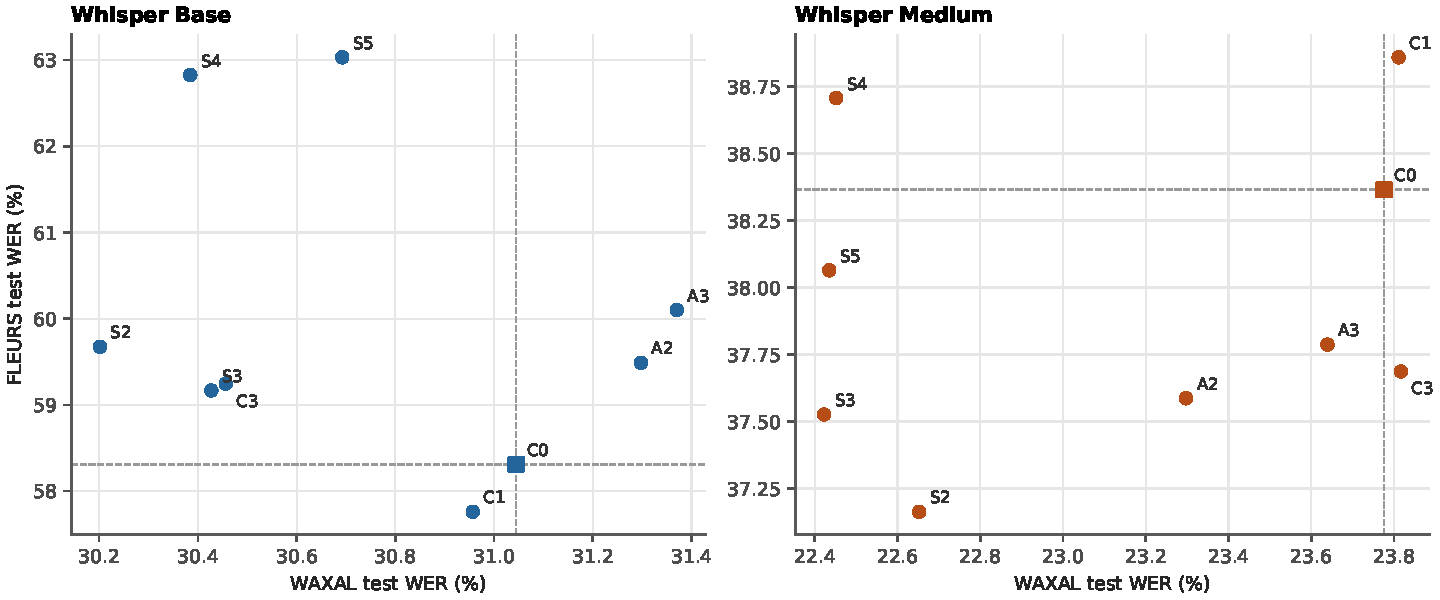
\includegraphics[width=\linewidth]{ch4_domain_scatter.pdf}
\caption{Mean WAXAL versus FLEURS test WER for each condition. Dashed lines pass
through the C0 control (square); points below and to the left of it are better
on both test sets. The axis ranges differ between panels.}
\label{fig:domain}
\end{figure}

\begin{table}[htbp]\centering\small
\caption{FLEURS test results (\%), mean $\pm$ SD over three seeds.
$\dagger$:~a single model. Base C3 is the mean of three evaluation exports
from that model.}
\label{tab:fleurs}
\begin{tabular}{lrrrr}\toprule
 & \multicolumn{2}{c}{Whisper Base} & \multicolumn{2}{c}{Whisper Medium}\\
\cmidrule(lr){2-3}\cmidrule(lr){4-5}
Code & WER & CER & WER & CER\\\midrule
% BEGIN AUTO fleurs
C0 & $58.31 \pm 0.59$ & $18.93 \pm 0.26$ & $38.36 \pm 0.48$ & $9.98 \pm 0.47$ \\
C1 & $57.76 \pm 0.05$ & $19.17 \pm 0.32$ & $38.86 \pm 0.58$ & $10.70 \pm 0.35$ \\
C3 & $59.25^{\dagger}$ & $20.09^{\dagger}$ & $37.69^{\dagger}$ & $9.93^{\dagger}$ \\
A2 & $59.49 \pm 1.47$ & $20.03 \pm 0.42$ & $37.59 \pm 0.44$ & $10.08 \pm 0.36$ \\
A3 & $60.10 \pm 2.04$ & $20.56 \pm 1.60$ & $37.79 \pm 0.65$ & $10.01 \pm 0.28$ \\
S2 & $59.67 \pm 0.51$ & $20.47 \pm 0.34$ & $37.16 \pm 0.28$ & $9.89 \pm 0.15$ \\
S3 & $59.17 \pm 1.03$ & $20.16 \pm 0.88$ & $37.53 \pm 0.27$ & $10.09 \pm 0.27$ \\
S4 & $62.83 \pm 1.10$ & $22.21 \pm 0.93$ & $38.71 \pm 1.34$ & $11.82 \pm 0.92$ \\
S5 & $63.03 \pm 1.24$ & $22.55 \pm 1.29$ & $38.06 \pm 0.29$ & $10.98 \pm 0.51$ \\
% END AUTO fleurs
\bottomrule\end{tabular}
\end{table}

Character and word error rates did not always agree. Medium A2 improved FLEURS
WER by 0.78~pp but CER worsened slightly (9.98\% to 10.08\%). Medium C1 worsened
FLEURS CER by 0.72~pp but WER by only 0.49~pp. In an agglutinative language, a
single wrong affix makes the whole word incorrect. WER and CER therefore weigh
small morphological errors differently, and they can rank the conditions
differently.

\subsection{Answer to RQ2}

Combining a curriculum with augmentation did not improve out-of-domain
generalisation beyond what augmentation achieved alone. None of the curriculum
and augmentation combinations, nor their interactions, differed measurably from
the corresponding augmentation-only condition. For Medium, neither combination
improved FLEURS WER; for Base, S3 improved on S2 externally (0.51~pp) but was
worse in-domain. Augmentation alone did help Whisper Medium. Light
spectrogram masking with random order gave the lowest external error (37.16\%,
1.20~pp better than C0) and was the only intervention whose in-domain benefit
survived adjustment for multiple comparisons. For Whisper Base, no augmentation
policy improved external recognition. The value of augmentation therefore
depended on the model as well as on the evaluation corpus.

\section{Computational cost}
\label{sec:cost}

Figure~\ref{fig:runtime} divides the recorded training time into training
updates and the three end-of-epoch validation passes used to select checkpoints.

\begin{figure}[htbp]\centering
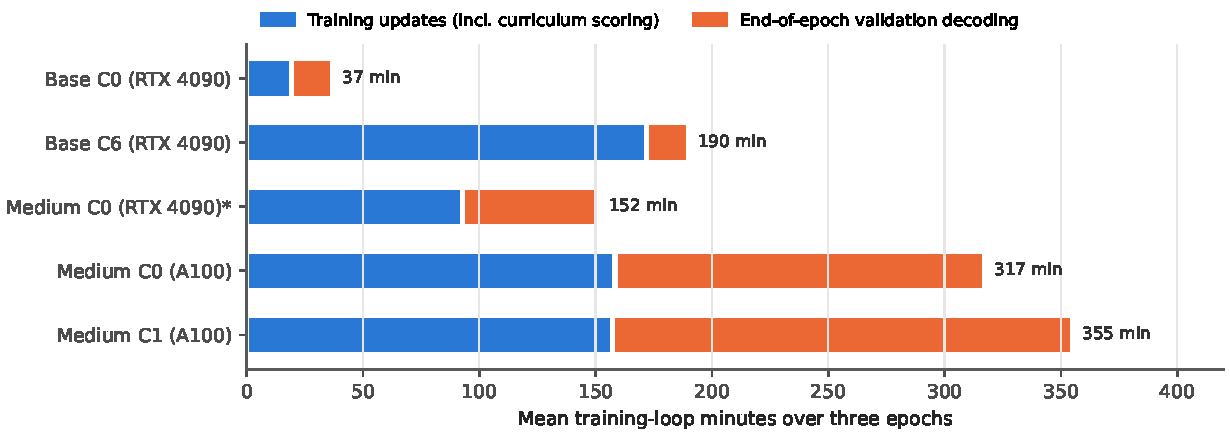
\includegraphics[width=0.9\linewidth]{ch4_runtime.pdf}
\caption{Mean recorded training-loop time, divided into training updates
(including any curriculum scoring) and end-of-epoch validation decoding.
*~Original Medium runs on the RTX~4090, repeated on the A100 for all reported
Medium results (Chapter~3).}
\label{fig:runtime}
\end{figure}

\begin{itemize}
\item \textbf{Static curricula and augmentation cost almost nothing.} Every
static curriculum and augmentation condition trained in about the same time as
its control (Appendix Table~\ref{tab:time}).
\item \textbf{SortaGrad's extra time is validation, not training.} On Medium,
SortaGrad conditions took 20--38 minutes longer. This is almost entirely the
slower validation decoding of the degraded epoch-1 model.
\item \textbf{The WER-based curriculum is expensive.} C6 must decode the whole
training set at each epoch to re-score it, raising Base training time from
37~to 190~minutes (5.1$\times$) without improving accuracy.
\end{itemize}

Medium training on the A100 took 317~minutes. About half of this was
validation decoding, and the training updates alone took longer than the same
updates on the RTX~4090 (158 versus 93~minutes). Because GPU, host machine and
concurrent workload changed together, this difference should not be read as
a property of the GPUs. Peak sampled device memory for Medium was
16.3--16.8~GiB, which confirms that the batch-size-six configuration fits
comfortably on either GPU.

\section{Summary of findings}
\label{sec:summary}

Table~\ref{tab:summary} maps each finding to its research question and to the
strength of the supporting evidence.

\begin{table}[htbp]\centering\small
\caption{Summary of findings. Intervals are 95\% paired cluster-bootstrap
intervals for Whisper Medium (pp; positive favours the treatment).}
\label{tab:summary}
\begin{tabularx}{\linewidth}{@{}p{0.2\linewidth}X p{0.17\linewidth}@{}}\toprule
Question & Finding & Evidence\\\midrule
RQ1: static curricula & No reliable change in final WER on either test set or
  for either model; a gain on one test set came with a loss on the other. &
  Medium WAXAL C1 $-0.04$ $[-0.36, 0.38]$, C3 $-0.04$ $[-0.40, 0.41]$\\
RQ1: dynamic curricula & Less accurate than random order (Base) and up to
  5.1$\times$ the training time. & Three seeds; descriptive\\
RQ1: training dynamics & SortaGrad severely degrades the model after epoch~1;
  C3 converges faster early; neither advantage persists. & All runs\\
RQ1: difficult utterances & No curriculum benefit on low-SNR or long
  utterances. & Figure~\ref{fig:bins}\\
RQ2: augmentation alone & Light masking improves Medium in-domain and
  externally; waveform augmentation probably helps Medium; neither helps Base
  externally. & S2: WAXAL $+1.12$ $[0.56, 1.57]$, FLEURS $+1.20$ $[0.37,
  2.00]$\\
RQ2: curriculum + augmentation & No added benefit over augmentation alone;
  no interaction distinguishable from zero. & Four interaction intervals all
  include 0\\
RQ2: masking strength & Stronger masking reduces external accuracy. & S4 vs S2
  FLEURS $-1.54$ $[-2.83, -0.44]$\\\bottomrule
\end{tabularx}
\end{table}

\section{Limitations}
\label{sec:limitations}

\begin{itemize}
\item \textbf{Training variation.} Three seeds give limited information about
variation between training runs, and the bootstrap intervals do not include it.
With three paired runs, an exact sign test cannot give a two-sided $p$ below
0.25. Claims about run-to-run consistency therefore rest on the direction of
the three seeds, not on a formal test.
\item \textbf{Fixed budget.} Most runs were still improving at epoch~3. Longer
training could change the size, and possibly the direction, of effects that
act late in training, such as regularisation by masking.
\item \textbf{Selection of the combined curriculum.} C3 was chosen as the
curriculum to combine with waveform augmentation after the Base screening
results had been inspected. The combined comparisons therefore do not form a
fully pre-specified test.
\item \textbf{Base--Medium comparison.} Model size and GPU differ together
between the two models (Section~\ref{sec:reading}).
\item \textbf{Truncation.} Utterances longer than 30~seconds (2.4\% of the WAXAL
test set) are truncated while their full transcript is kept, which inflates
deletions for those utterances in every condition alike.
\item \textbf{External clusters.} FLEURS speaker identities were not available,
so its intervals resample sentence prompts and may understate dependence
between recordings by the same speaker.
\item \textbf{Planned but not run.} The isolated waveform-augmentation
conditions described in Chapter~3 (noise only, reverberation only, tempo only,
and their conditional combination), and the uniform difficulty mixing for the
dynamic curricula, were not run within the available compute budget. The
waveform results therefore cannot be attributed to any single transformation,
and the dynamic curricula were evaluated without mixing. These are natural
next steps.
\end{itemize}

\appendix
\renewcommand{\thesection}{\thechapter.\Alph{section}}
\section{Supplementary tables}

\begin{table}[htbp]\centering\scriptsize
\caption{Matched test-WER differences (control minus treatment, pp), with 95\%
paired cluster-bootstrap intervals for Whisper Medium. Values correspond to
Figure~\ref{fig:forest}.}
\label{tab:effects}
\begin{tabular}{lrrrr}\toprule
 & \multicolumn{2}{c}{WAXAL} & \multicolumn{2}{c}{FLEURS}\\
\cmidrule(lr){2-3}\cmidrule(lr){4-5}
Comparison & Base & Medium & Base & Medium\\\midrule
% BEGIN AUTO effects
C1 vs C0 & $+0.09$ & $-0.04\;[-0.36, +0.38]$ & $+0.55$ & $-0.49\;[-1.35, +0.28]$ \\
C3 vs C0 & $+0.59$ & $-0.04\;[-0.40, +0.41]$ & $-0.94$ & $+0.68\;[-0.15, +1.52]$ \\
A2 vs C0 & $-0.25$ & $+0.48\;[-0.04, +0.89]$ & $-1.18$ & $+0.78\;[-0.01, +1.59]$ \\
A3 vs C3 & $-0.91$ & $+0.18\;[-0.43, +0.67]$ & $-0.85$ & $-0.10\;[-0.99, +0.77]$ \\
A3 vs A2 & $-0.07$ & $-0.34\;[-0.84, +0.30]$ & $-0.61$ & $-0.20\;[-0.98, +0.56]$ \\
S2 vs C0 & $+0.84$ & $+1.12\;[+0.56, +1.57]$ & $-1.36$ & $+1.20\;[+0.37, +2.00]$ \\
S3 vs C1 & $+0.53$ & $+1.39\;[+0.93, +1.71]$ & $-1.41$ & $+1.33\;[+0.40, +2.28]$ \\
S3 vs S2 & $-0.23$ & $+0.23\;[-0.09, +0.56]$ & $+0.51$ & $-0.36\;[-0.98, +0.24]$ \\
S4 vs S2 & $-0.18$ & $+0.20\;[-0.35, +0.68]$ & $-3.15$ & $-1.54\;[-2.83, -0.44]$ \\
S5 vs S3 & $-0.27$ & $-0.01\;[-0.52, +0.37]$ & $-3.87$ & $-0.54\;[-1.62, +0.41]$ \\
% END AUTO effects
\bottomrule\end{tabular}
\end{table}

\begin{table}[htbp]\centering\small
\caption{Whisper Base curriculum conditions (\%, minutes). $\dagger$:~a single
model.}
\label{tab:base-curricula}
\begin{tabular}{lrrrrr}\toprule
Code & WAXAL val.\ WER & WAXAL test WER & WAXAL test CER & FLEURS test WER & Minutes\\\midrule
% BEGIN AUTO basecur
C0 & $32.91 \pm 0.48$ & $31.04 \pm 0.29$ & $6.82 \pm 0.17$ & $58.31 \pm 0.59$ & $37.2 \pm 0.5$ \\
C1 & $32.60 \pm 0.11$ & $30.96 \pm 0.06$ & $6.89 \pm 0.12$ & $57.76 \pm 0.05$ & $38.3 \pm 1.1$ \\
C2 & $33.12^{\dagger}$ & $31.53^{\dagger}$ & $7.46^{\dagger}$ & $60.56^{\dagger}$ & $37.8 \pm 1.0$ \\
C3 & $32.84^{\dagger}$ & $30.46^{\dagger}$ & $6.47^{\dagger}$ & $59.25^{\dagger}$ & $37.7 \pm 0.9$ \\
C5 & $33.91 \pm 0.26$ & $31.78 \pm 0.73$ & $7.37 \pm 0.68$ & $60.39 \pm 0.97$ & $47.8 \pm 16.8$ \\
C6 & $33.92 \pm 0.33$ & $31.98 \pm 0.28$ & $6.93 \pm 0.10$ & $58.91 \pm 0.93$ & $189.9 \pm 38.5$ \\
% END AUTO basecur
\bottomrule\end{tabular}
\end{table}

\begin{table}[htbp]\centering\small
\caption{Training-loop minutes (mean $\pm$ SD), including end-of-epoch
validation. Base: RTX~4090; Medium: A100.}
\label{tab:time}
\begin{tabular}{lrr}\toprule
Code & Whisper Base & Whisper Medium\\\midrule
% BEGIN AUTO time
C0 & $37.2 \pm 0.5$ & $317.3 \pm 1.4$ \\
C1 & $38.3 \pm 1.1$ & $355.2 \pm 4.1$ \\
C3 & $37.7 \pm 0.9$ & $314.0 \pm 0.8$ \\
A2 & $37.5 \pm 0.2$ & $315.5 \pm 0.7$ \\
A3 & $37.1 \pm 0.7$ & $316.5 \pm 1.5$ \\
S2 & $38.1 \pm 1.1$ & $316.3 \pm 0.6$ \\
S3 & $38.7 \pm 0.8$ & $339.3 \pm 6.4$ \\
S4 & $37.5 \pm 0.4$ & $317.4 \pm 1.7$ \\
S5 & $38.0 \pm 0.8$ & $337.7 \pm 2.0$ \\
C5 & $47.8 \pm 16.8$ & -- \\
C6 & $189.9 \pm 38.5$ & -- \\
% END AUTO time
\bottomrule\end{tabular}
\end{table}

\begin{table}[htbp]\centering\small
\caption{Whisper Medium WAXAL test WER (\%) for the original RTX~4090 runs and
their A100 repetitions (same seed). Positive differences mean the A100 run had
lower WER. All Medium results in this chapter use the A100 runs.}
\label{tab:migration}
\begin{tabular}{llrrr}\toprule
Code & Seed & RTX 4090 & A100 & Difference (pp)\\\midrule
% BEGIN AUTO migration
C0 & 42 & 24.24 & 24.14 & +0.09 \\
C0 & 43 & 23.59 & 23.56 & +0.03 \\
C0 & 44 & 23.95 & 23.62 & +0.33 \\
C1 & 42 & 23.66 & 24.17 & -0.51 \\
C1 & 43 & 23.81 & 23.64 & +0.17 \\
% END AUTO migration
\bottomrule\end{tabular}
\end{table}

\begin{thebibliography}{9}
\bibitem[Amodei et~al.(2016)]{Amodei2015}
Amodei, D., et~al. (2016). Deep Speech 2: End-to-end speech recognition in
English and Mandarin. \emph{Proceedings of ICML}.
\url{https://arxiv.org/abs/1512.02595}.
\bibitem[Bengio et~al.(2009)]{Bengio2009}
Bengio, Y., Louradour, J., Collobert, R., and Weston, J. (2009).
Curriculum learning. \emph{Proceedings of ICML}.
\url{https://doi.org/10.1145/1553374.1553380}.
\bibitem[Park et~al.(2019)]{Park2019}
Park, D.~S., et~al. (2019). SpecAugment: A simple data augmentation method
for automatic speech recognition. \emph{Proceedings of Interspeech}, 2613--2617.
\url{https://doi.org/10.21437/Interspeech.2019-2680}.
\end{thebibliography}
\end{document}
